% t = top align slides, alternative c = center
% handout/final = bullet points etc. one by one (final) or all on the slide immediately (handout)
\documentclass[t,xcolor={dvipsnames},final,aspectratio=169]{beamer}
\beamertemplatenavigationsymbolsempty
\usepackage{adjustbox}
%\setbeameroption{hide notes}
\setbeameroption{show notes on second screen}

\mode<presentation> {
	\usetheme{Frankfurt}
	\usecolortheme{crane}
	\setbeamertemplate{footline}[frame number]
	\beamerdefaultoverlayspecification{<+->}
}

\title{How (not?) to use Large Language Models}

\author{Pablo Mosteiro}
\institute[UU]{
Utrecht University: Welfare, Participation and Citizenship in a Digital World
}
\date{2025-09-25}
\logo{
\includegraphics[scale=0.5]{img/UU-logo2011_CMYK-eps-converted-to.pdf}\hspace*{0.65\textwidth}\vspace{-8mm}}
\begin{document}
\begin{frame}
\maketitle
\end{frame}

{\setbeamertemplate{logo}{}
\begin{frame}
\frametitle{Table of Contents}
\tableofcontents
\end{frame}
}

\section{What is an LLM}
\begin{frame}{}
\huge{What is an LLM}
\end{frame}
\begin{frame}{How are they trained?}
\begin{itemize}
\item What do you think is the next word that I will...?
\end{itemize}
\end{frame}
\begin{frame}{How are they trained?}
\begin{itemize}
\item What do you think is the next word that I will WRITE?
\item What do you think is the next word that I will SAY?
\item How did you guess?
\end{itemize}
\end{frame}

\begin{frame}{LLMs as coding agents}
\texttt{a = [2, 4, 5]}
\pause

\texttt{\# Compute the mean of the list}
\pause

Can the LLM auto-complete?
\end{frame}

{\setbeamertemplate{logo}{}
\begin{frame}{LLMs as bug fixers}
\texttt{\# Create a dictionary with elements in the name of a person}
\texttt{name\_parts = \{"given name": "Consolacion", "surname": "Valenzuela"\}} \\
\texttt{\# Add a middle name}\\
\texttt{name\_parts.append("middle name": "Celestina")}

\pause
\vfill
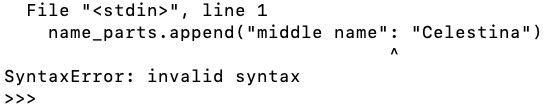
\includegraphics[width=8cm]{img/error.png}

\pause
\vfill
\includegraphics<+->[width=8cm]{img/llm.png}
\end{frame}
}

\section{Ethics}
\begin{frame}{}
\huge{How (or why) \textbf{not} to use LLMs}
\end{frame}

\begin{frame}{Training data}
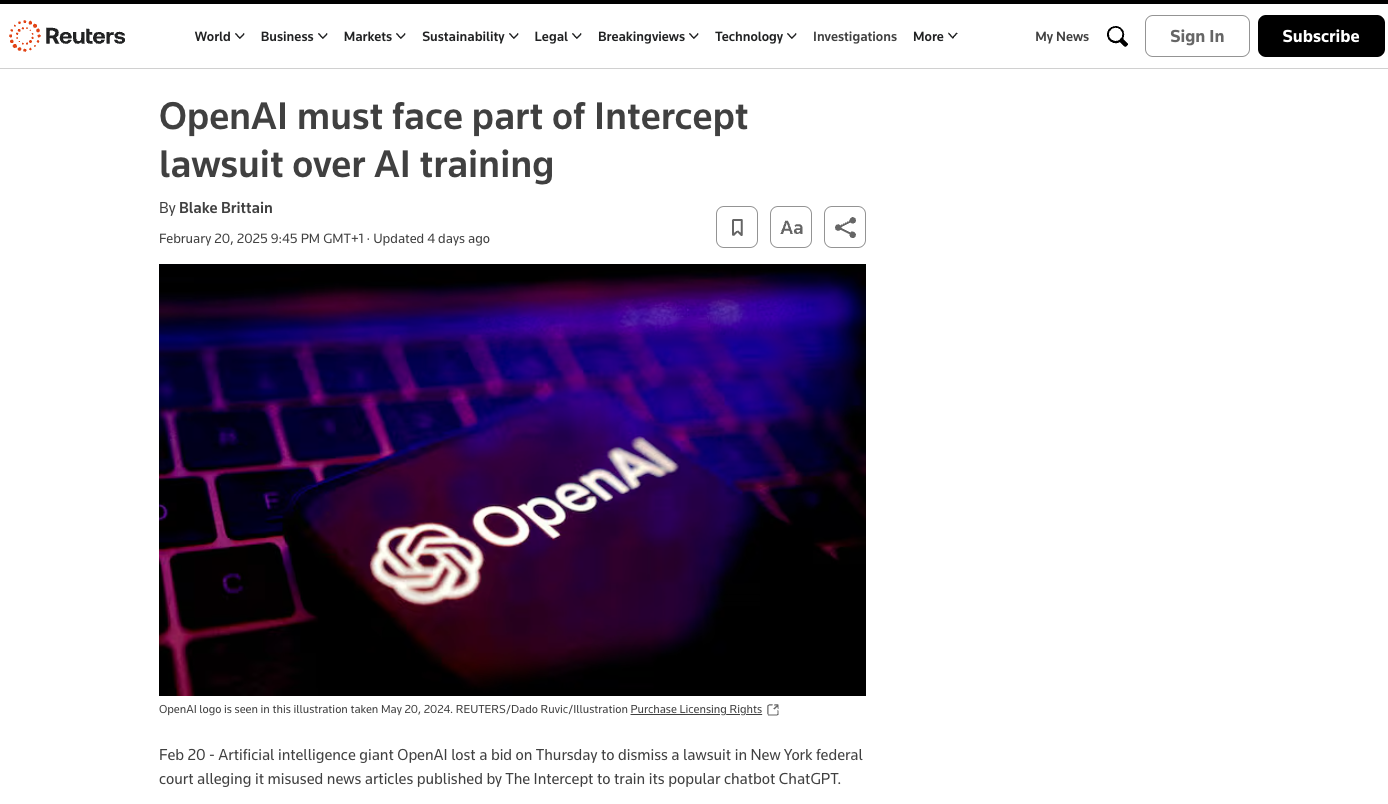
\includegraphics[width=\textwidth]{img/trainingdata.png}
  \note{
  Unethical and possibly illegal access to data\\
  
  No open-source principles $\rightarrow$ no explainability, no reproducibility
  }
\end{frame}

{\setbeamertemplate{logo}{}
\begin{frame}{Environment}
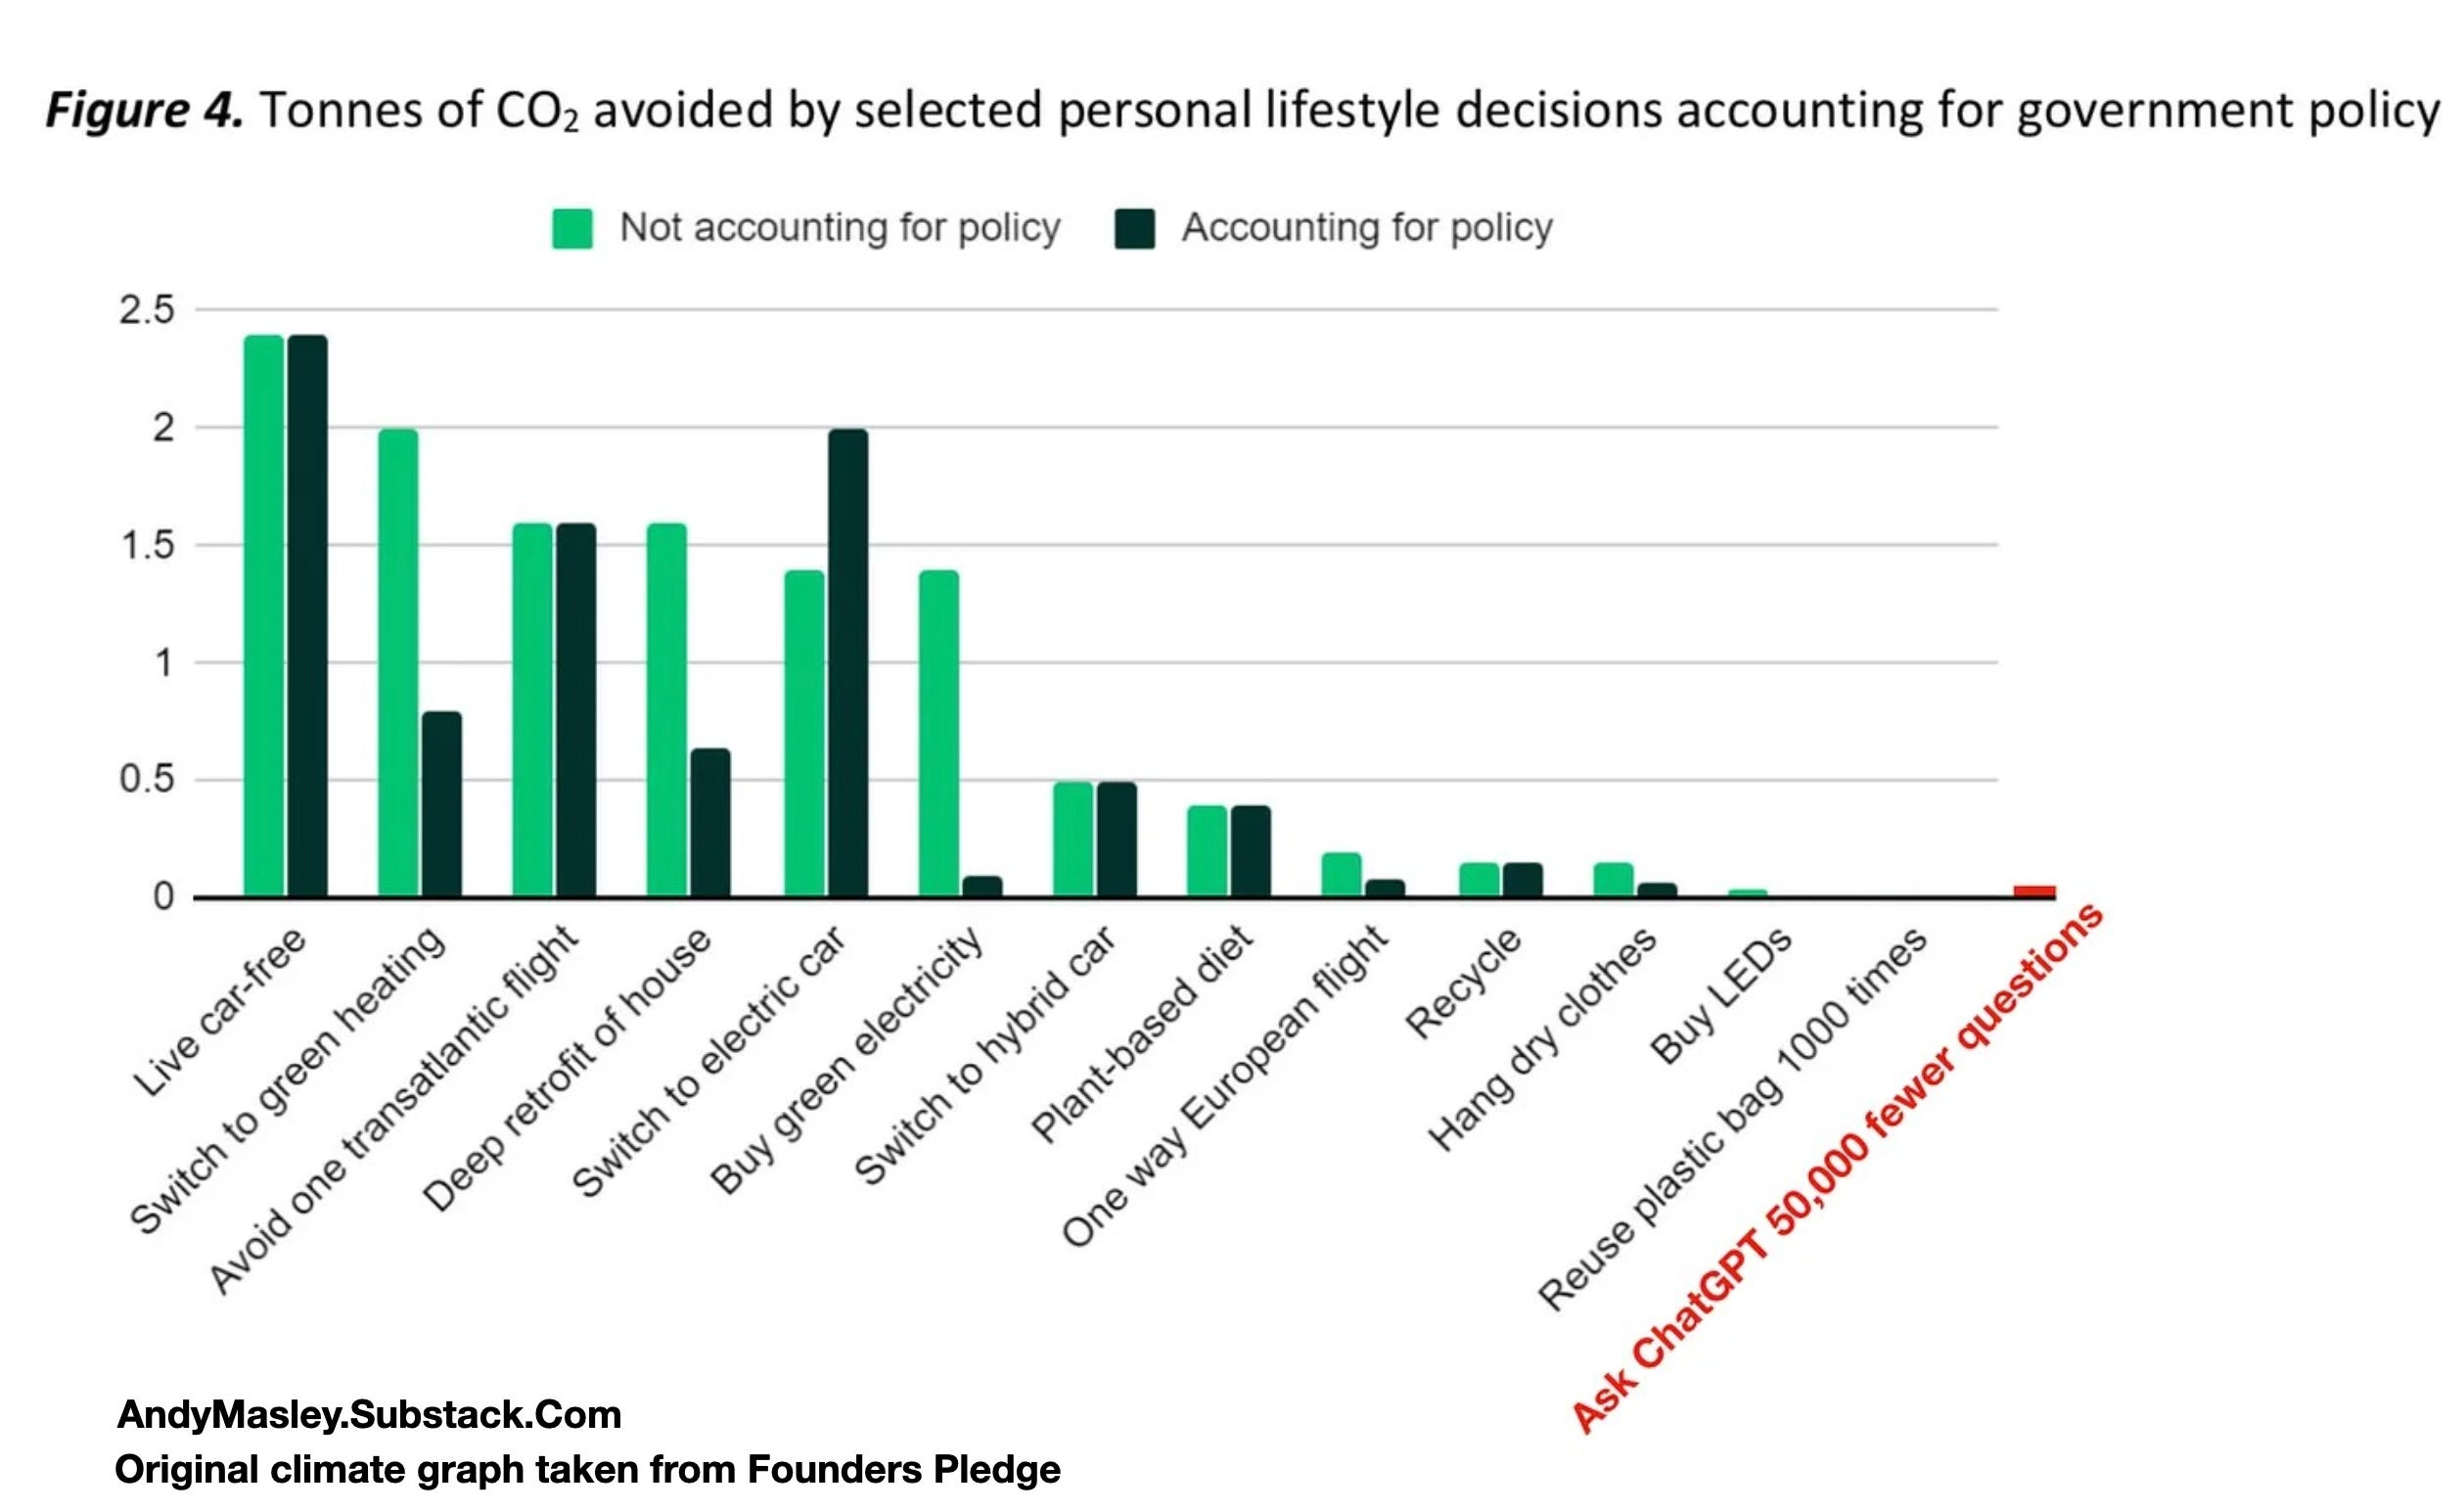
\includegraphics[width=0.7\textwidth]{img/emissions.jpg}
\footnote{Source (January 2025): \url{https://open.substack.com/pub/andymasley/p/individual-ai-use-is-not-bad-for}}
\end{frame}
}

{\setbeamertemplate{logo}{}
\begin{frame}{Labor conditions}
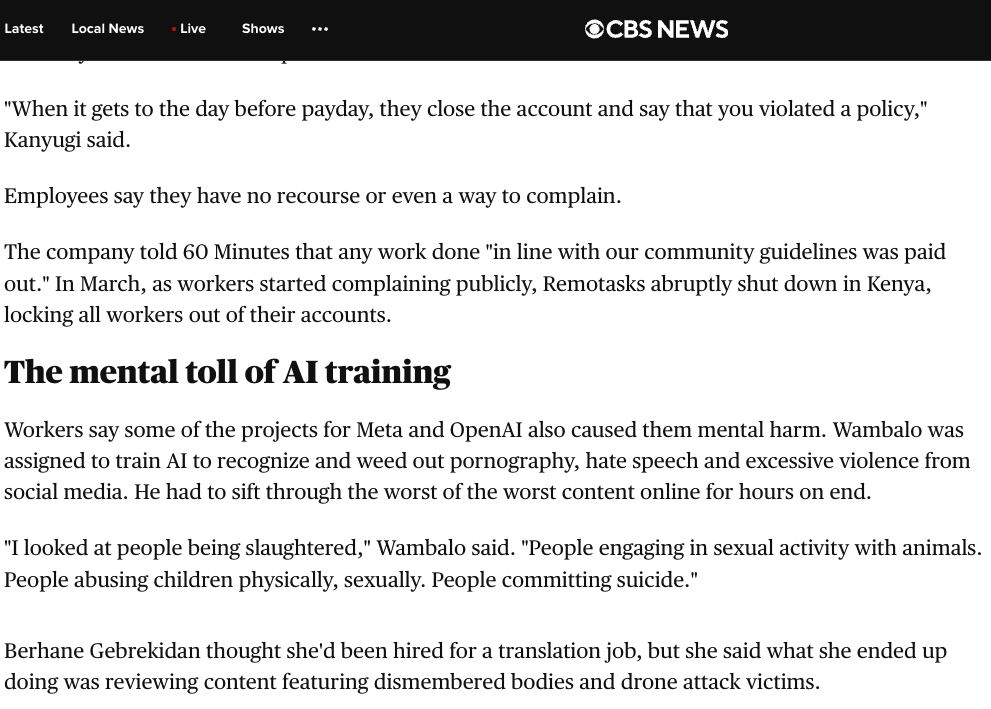
\includegraphics[width=0.6\textwidth]{img/labor.png}
\footnote{Source (November 2024): \url{https://www.cbsnews.com/news/ai-work-kenya-exploitation-60-minutes/}}
\end{frame}
}

{\setbeamertemplate{logo}{}
\begin{frame}{Effect on cognition}
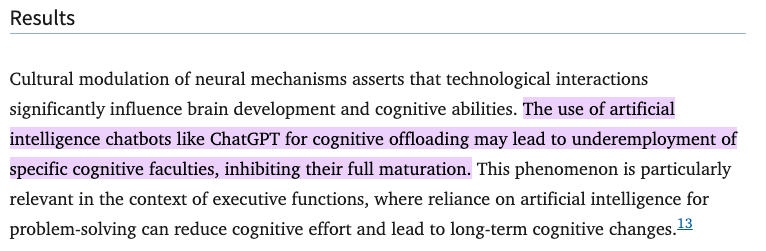
\includegraphics[width=0.6\textwidth]{img/cognition.png}
\footnote{Source (June 2024): Dubey et al. Redefining Cognitive Domains in the Era of ChatGPT: A Comprehensive Analysis of Artificial Intelligence's Influence and Future Implications. Med Res Arch. 2024 Jun;12(6):5383. doi: 10.18103/mra.v12i6.5383}
\end{frame}
}

\begin{frame}{Uploading restricted data}
\includegraphics<+->[width=8cm]{img/llm.png}
\begin{itemize}
\item What if error contains sensitive information?
\end{itemize}
\includegraphics<+->[width=8cm]{img/municipalitiescode.png}
\includegraphics<+->[width=8cm]{img/municipalitieserror.png}
\end{frame}

%\begin{frame}{Uploading restricted data}
%\includegraphics<+->[width=8cm]{img/municipalitiescode.png}
%\includegraphics<+->[width=8cm]{img/municipalitieserror.png}
%\includegraphics<+->[width=8cm]{img/llm.png}
%\begin{itemize}
%\item Corrected code is useless / does not work
%\end{itemize}
%\end{frame}

\begin{frame}{Uploading restricted data}
\includegraphics<+->[width=8cm]{img/llmdata.png}
\begin{itemize}
\item May be illegal!
\end{itemize}
\end{frame}

\section{Alternatives}

\begin{frame}{}
\huge{Alternatives}
\end{frame}

{\setbeamertemplate{logo}{}
\begin{frame}{HuggingChat}
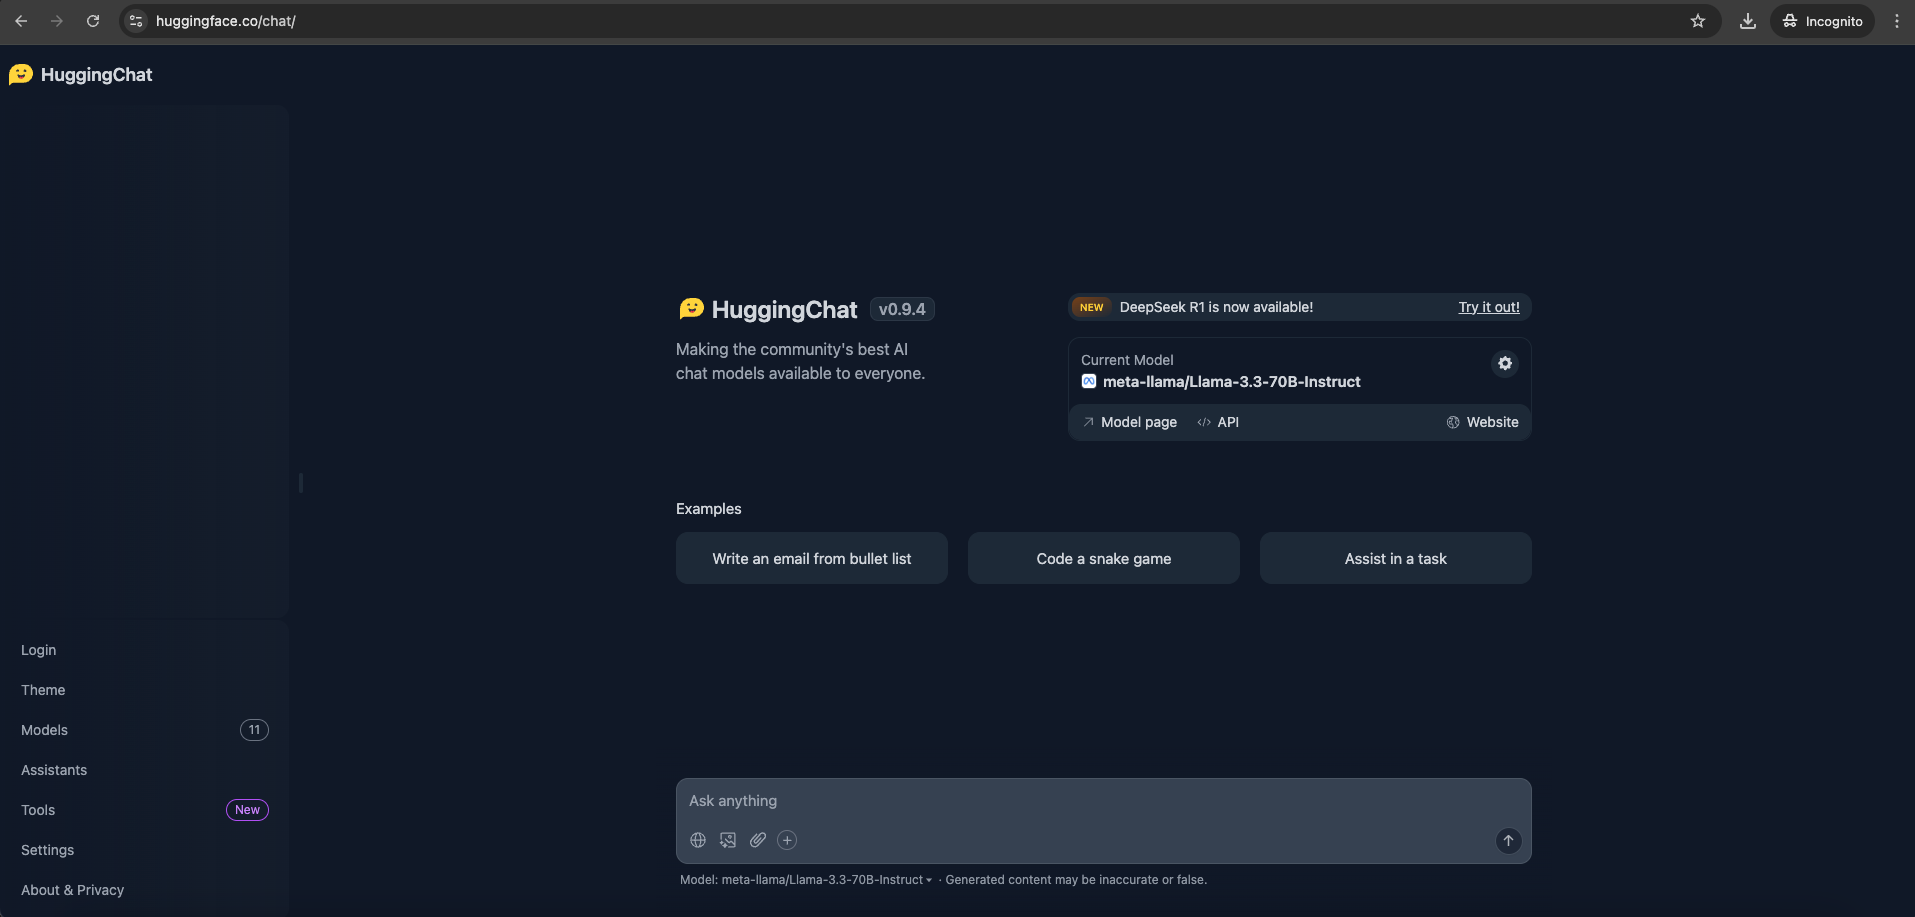
\includegraphics[width=0.9\textwidth]{img/huggingchat.png}
\end{frame}
}

\begin{frame}{Switch models}
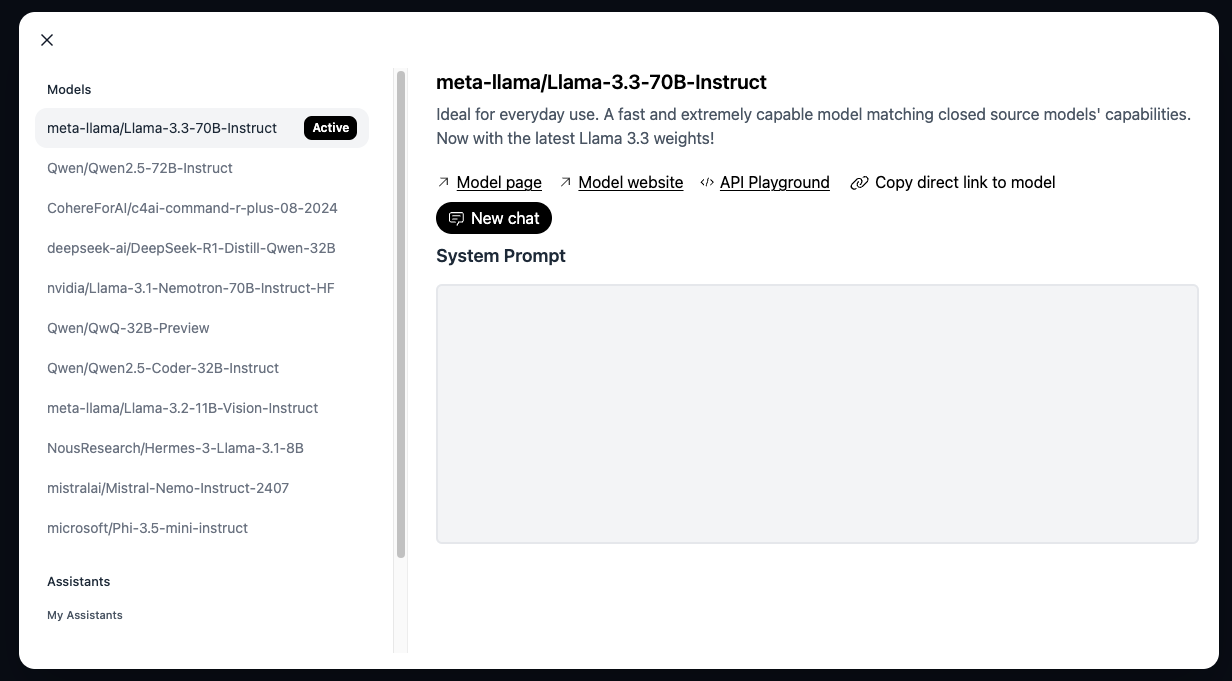
\includegraphics[width=0.9\textwidth]{img/models.png}
\end{frame}

{\setbeamertemplate{logo}{}
\begin{frame}{Unfortunately, ...}

\includegraphics[width=0.9\textwidth]{img/huggingchat_closed.png}
\end{frame}
}

{\setbeamertemplate{logo}{}
\begin{frame}{Unfortunately, ...}

\includegraphics[width=0.9\textwidth]{img/huggingchat_closed.png}
\begin{itemize}
\item BUT...
\end{itemize}
\end{frame}
}

%\section{Colab}
%{\setbeamertemplate{logo}{}
%\begin{frame}{Generative AI on Google Colab}
%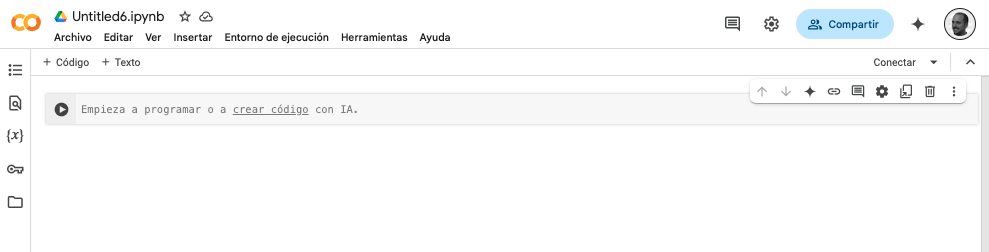
\includegraphics[width=0.8\textwidth]{img/colab.png}
%\pause
%\vfill
%
\includegraphics[width=0.5\textwidth]{img/gemini.png}
%\end{frame}
%}

%\begin{frame}{Model cards}
%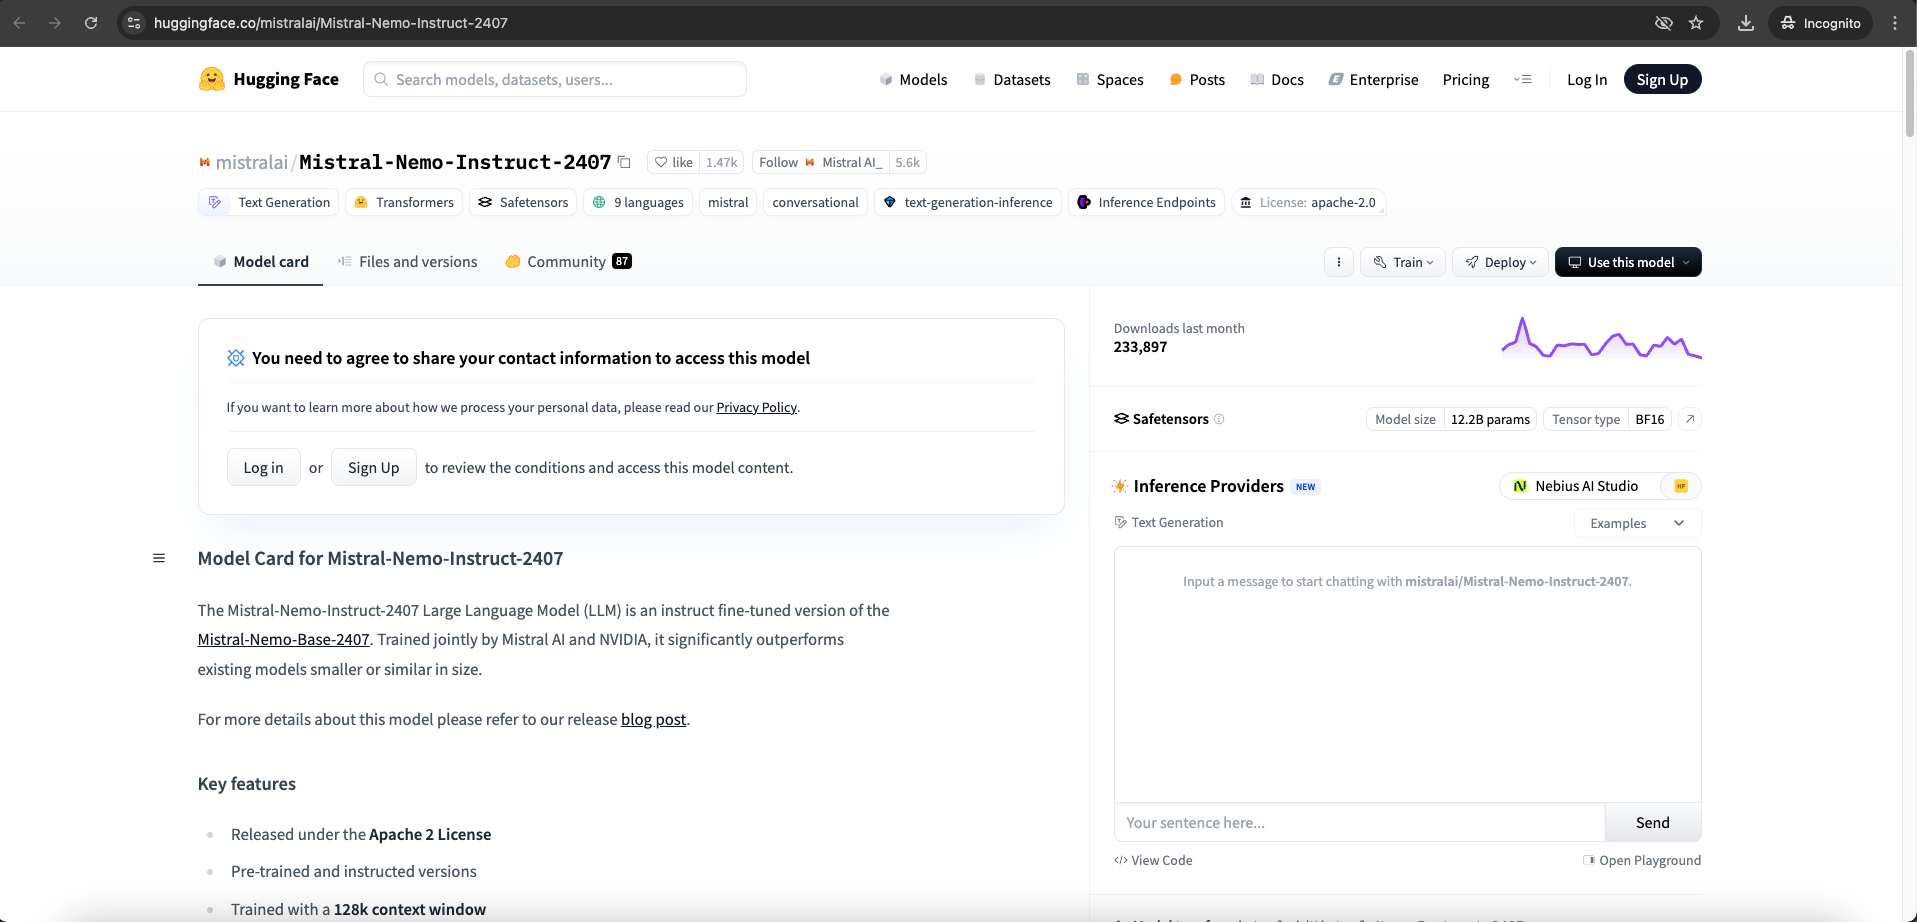
\includegraphics[width=0.7\textwidth]{img/modelcard.png}
%\pause

%No model card for Gemini!
%\end{frame}

{\setbeamertemplate{logo}{}
\begin{frame}{Using an LLM locally (no server)}
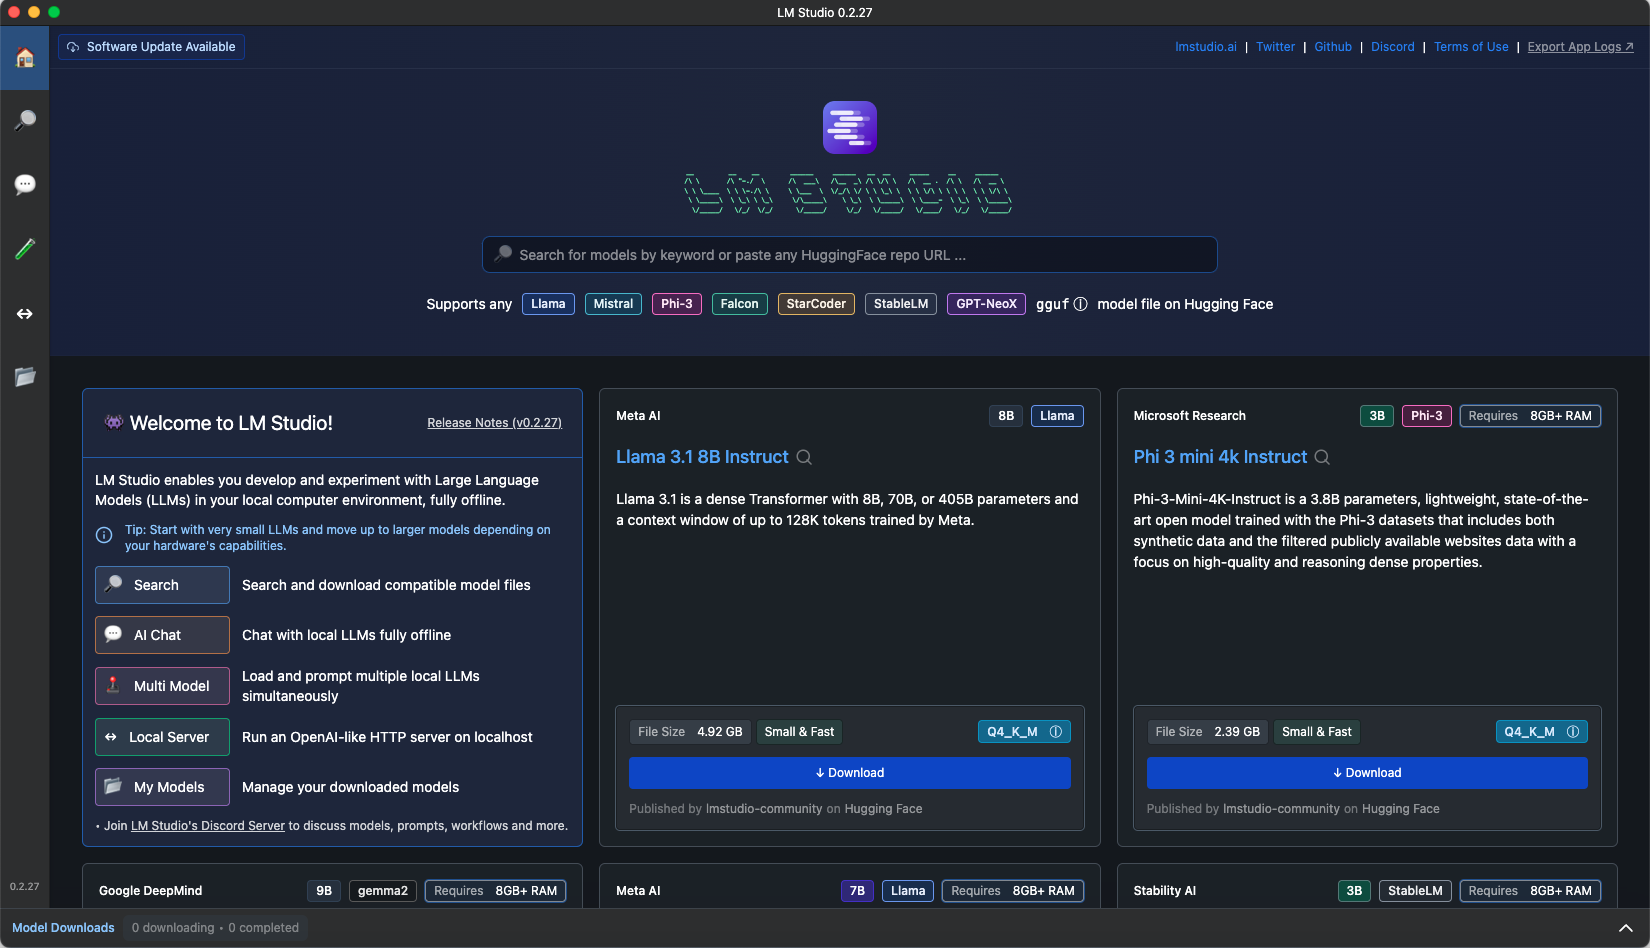
\includegraphics[width=0.8\textwidth]{img/lmstudio.png}
\note{But model can still be train in a very closed-source way}
\end{frame}
}

\begin{frame}{Versatile platform}
\begin{itemize}
\item \huge{OpenRouter.ai}
\item But before we do that...
\item Choose your poison carefully / Know what you choose
\item Do not share private data
\item Consider if you really need this
\end{itemize}
\end{frame}

\section{Application}
\begin{frame}{}
\huge{A practical application:\\

Sexism detection}
\end{frame}

\begin{frame}{Problem}
  \begin{columns}
    \begin{column}{0.45\textwidth}
    \begin{center}
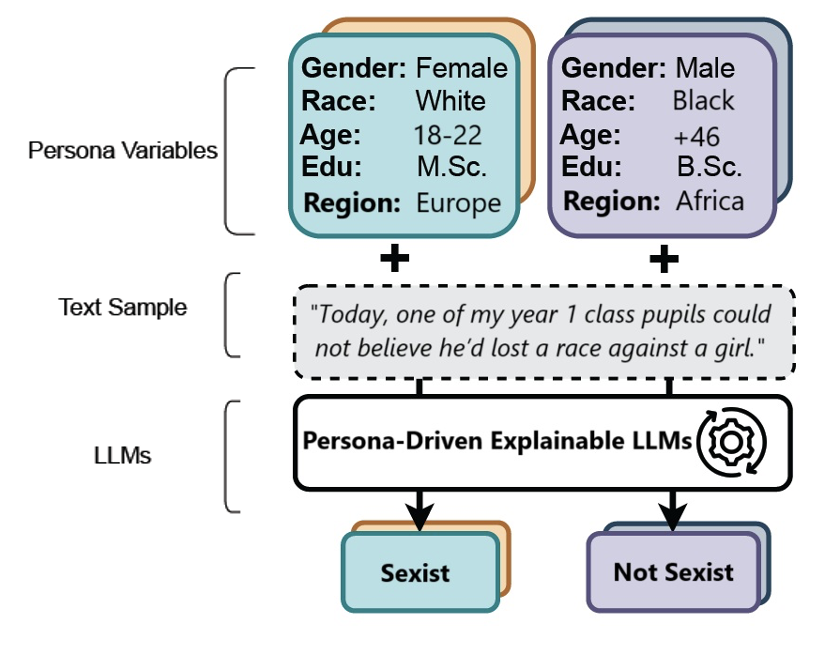
\includegraphics[width=0.9\textwidth]{img/problem.png}
\end{center}
    \end{column}
    \begin{column}{0.45\textwidth}  %%<--- here
\begin{itemize}
\item Reliable annotations are key to building strong NLP models
\item Some levels of disagreement are inevitable, particularly in subjective tasks
\item \textbf{This study: role of the annotator’s demographics features and text content in labeling decisions}
\end{itemize}
    \end{column}
  \end{columns}
\note{Can LLMs replace human annotators?}
\end{frame}

\begin{frame}{The paper}
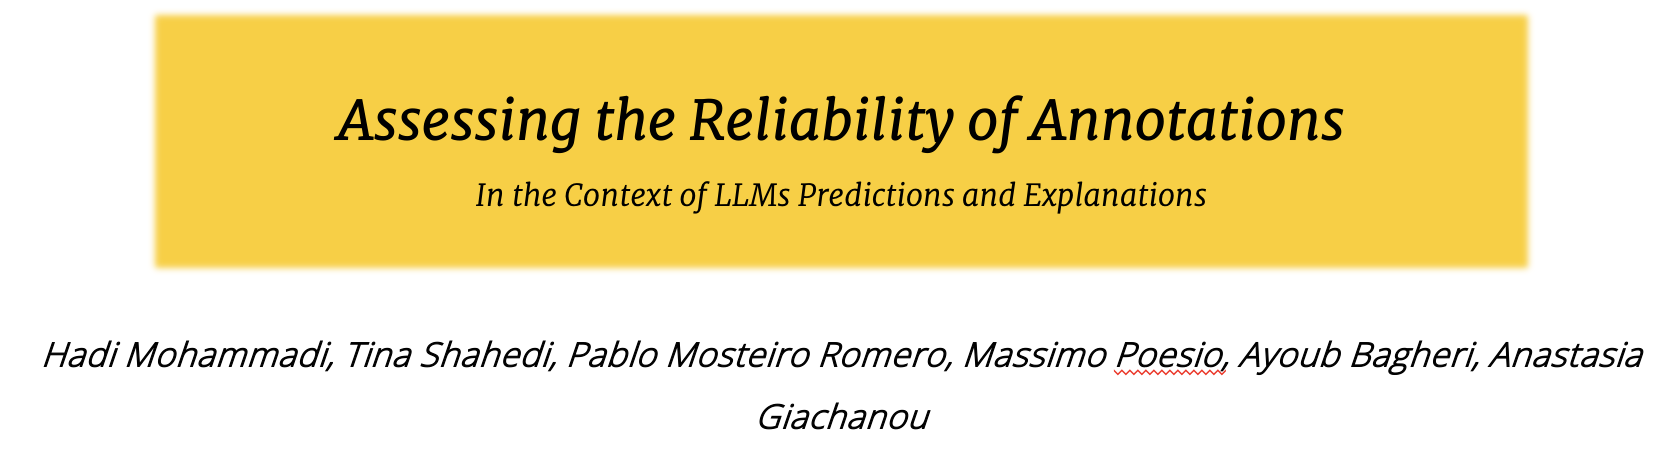
\includegraphics[width=0.9\textwidth]{img/credit.png}
\end{frame}

\begin{frame}{Data}
\begin{itemize}
\item We used data from the EXIST 2024 challenge — the sexism detection tasks.
\item  We focused on Task 1—classifying tweets as sexist or not.
\item Tweets in both English and Spanish
\item Each tweet in the dataset was annotated by six individuals.
\item The annotators' demographic features include:
\end{itemize}
\begin{center}
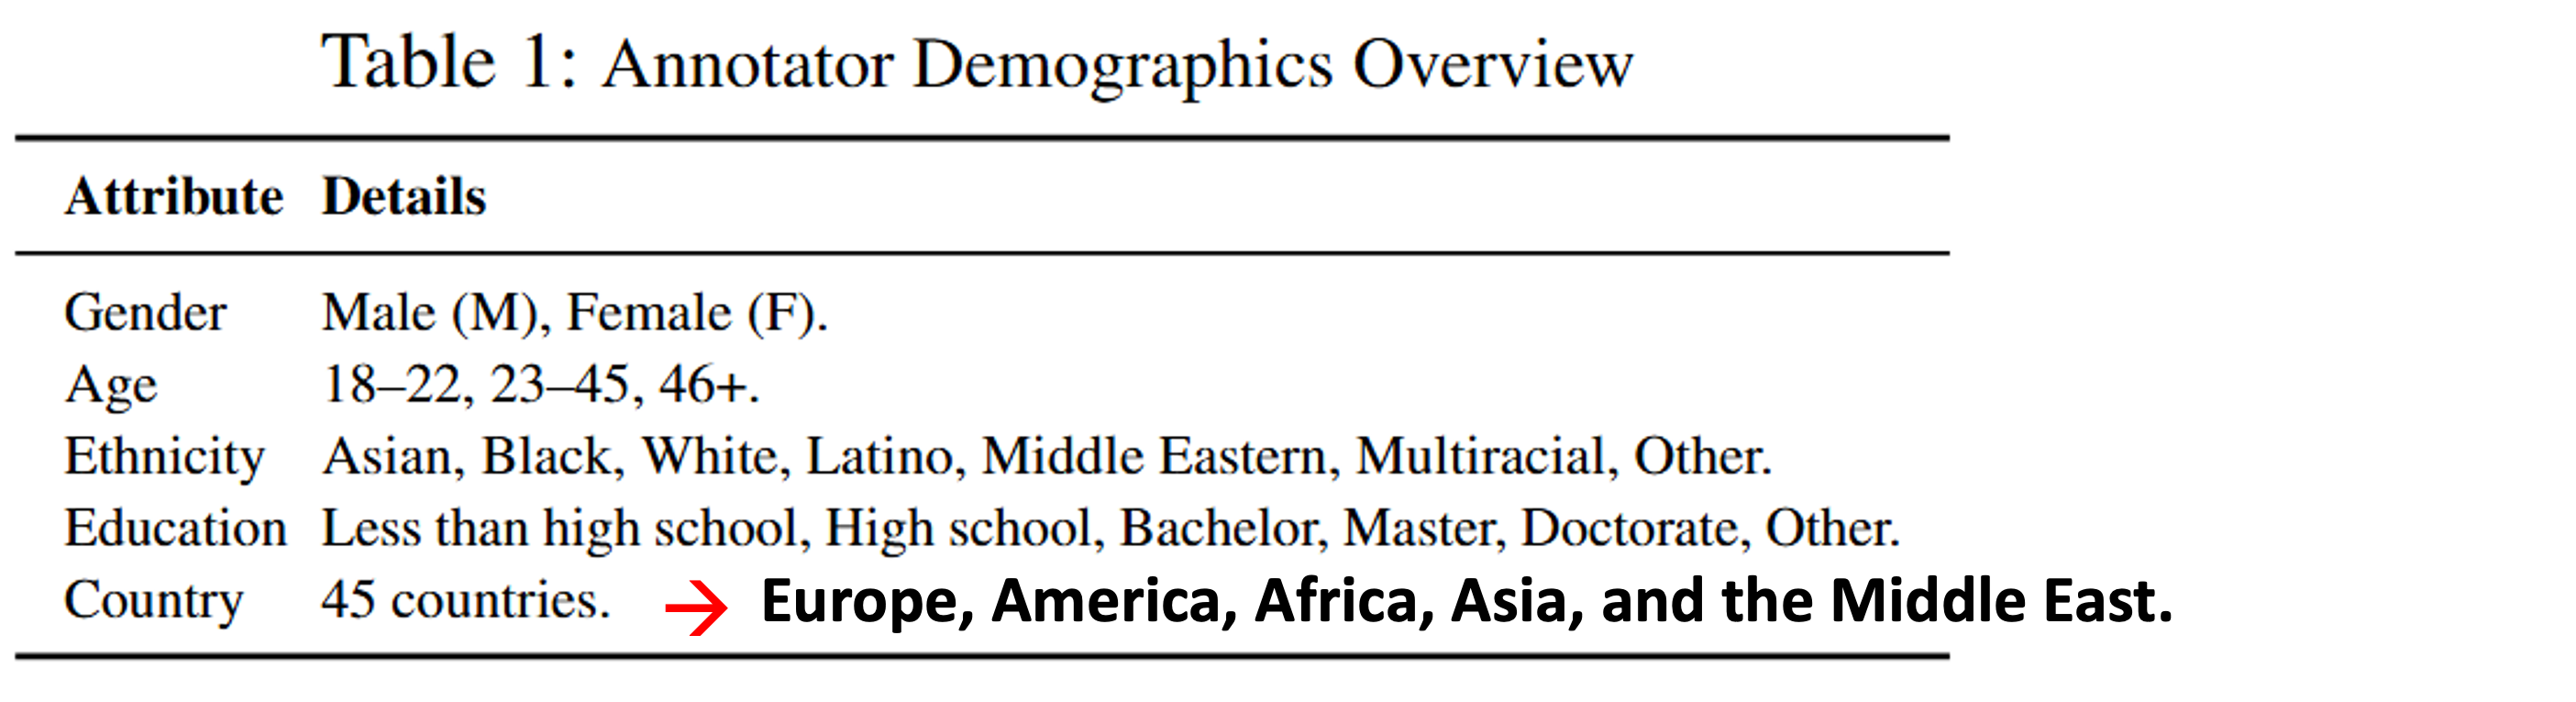
\includegraphics[width=0.7\textwidth]{img/demographics.png}
\end{center}
\end{frame}

\begin{frame}{Our objectives}
\begin{itemize}
\item Goal 1: Analyze the impact of demographic factors on annotation in the sexism detection task. 

\item Goal 2: Evaluate the potential of GenAI models to replace human annotators. 
\end{itemize}
\end{frame}

\end{document}
